\chapter{Fundamentação Teórica}

	De acordo com Oliveira e ANDRADE (2010), Sistemas embarcados são sistemas computacionais completos e independentes que possui a parte física (Hardware) e Lógica (Software ou Firmware), mais simples que um computador de propósito geral (Desktops), encarregados de executar apenas uma função determinada - tarefas pré-determinadas, com requisitos específicos, na qual executam geralmente repetidas vezes. Por serem muito simples, muitas vezes esses sistemas não têm flexibilidade (de software e de hardware) que lhes permita fazer outras tarefas quaisquer que não sejam aquelas para as quais foram desenhados e desenvolvidos.
Um grande responsável pela expansão do uso e aplicação dos sistemas embarcados foi a utilização do microcontrolador, pelo seu baixo custo, versatilidade e tamanho reduzido. Muitos microcontroladores podem ser conectados a dispositivos analógicos, permitindo o uso de sensores diversos. Isso permite a criação de dispositivos simples, que monitoram temperatura, umidade, entre outros fatores, executando ações predefinidas em caso de mudanças.
Em geral os sistemas embarcados possuem uma capacidade de processamento reduzida em comparação com computadores desktops. Ao invés de utilizar microprocessadores, os desenvolvedores preferem utilizar microcontroladores, pois estes já possuem diversos periféricos integrados no mesmo chip.V850, FR-V Outra diferença é a variedade de arquiteturas disponíveis tais como ARM, MIPS, Coldfire/68k, PowerPC, x86, PIC, 8051, Atmel AVR, Renesas H8, SH, M32R, Z80 e Z8.
Os sistemas embarcados comunicam-se com o meio externo através de periféricos. Estes periféricos podem ser combinados com o processador (como no caso dos sistemas microcontrolados) ou associados no sistema.
Entre os periféricos mais comum temos:
	Entrada de dados através de teclas (geralmente através de teclados feitos com varredura matricial)
Leds
	Displays de LCD (sendo os mais comuns os alfanuméricos por exemplo o HD44780)
Interface serial - (Por exemplo RS 232, I2C)
Universal Serial Bus - (USB)
TCP/IP

 

 

Hardware 
Graças a tecnologia baseada em transistores é possível miniaturizar componentes como os circuitos integrados, processadores e seus periféricos com baixo custo através de encapsulamento permitiu ter uma variedade de dispositivos para uma determinada aplicações e aperfeiçoa-la assim como os conversores analógico- digital (AD) capaz de digitalizar toda a informação em apenas uma fração de tempo.  Possui na sua arquitetura: Unidade Central de Processamento composto por unidade Logica e aritmética, Unidade de controle, Sistema de memória composto por memória de acesso aleatório e de Armazenamento e Sistemas de Entrada e saída interligados por meios de barramentos.
Firmware
É um tipo de Software Embarcado que controla o Hardware usando linguagens de baixo nível (Linguagem de máquina). Ele possui os principais componentes: Sistema básico de entrada e saída (BIOS) BASIC IMPUT OUTPUT SYSTEM serve parar inicializar o sistema, checar os dispositivos e carregar o Sistema Operacional (SO); SETUP responsável por alterar os parâmetros da memória de configuração (CMOS) que é usada para gravar as configurações do SETUP em uma pequena área de memória volátil alimentado por uma bateria. Podendo operar em tempo real onde determinadas tarefas tem o seu prazo compatíveis com a ocorrência dos eventos.
Controller Area Network (CAN)
Baseada em aplicações em tempo real um meio para transmissões de redes e controla o fluxo e propagação de mensagens sendo necessario um cotrole rígido de erro para que haja eficácia no recebimento de mensagens.
Godoy et al; 2010. Afirma que O CAN (Bosch, 2006) é um protocolo de comunicação digital serial e não determinístico, onde a comunicação de dados é baseada em mensagens formadas por quadros de bits com determinada função. Entre esses quadros de bits, existe o campo identificador (identifier ID) que caracteriza e define a prioridade de cada mensagem. O valor do identificador de uma mensagem em uma rede CAN é exclusivo e quanto mais baixo seu valor, maior será a prioridade da mensagem. Os sinais elétricos digitais do CAN são representados pelo nível recessivo (nível lógico 1) e nível dominante (nível lógico 0), sendo eles sinais diferenciais entre os dois fios da rede.(GODOY et al; 2010)

\label{cap:fundamentacao-teorica}



\section{Fundamentação Teórica A}

	
	\begin{figure}[h!]
		\centering
		\Caption{\label{fig:exemplo-2} Diagrama básico de um sistema embarcado dotado de um microcontrolador monitorando o ambiente.}	
		\UNIFORfig{}{
			\fbox{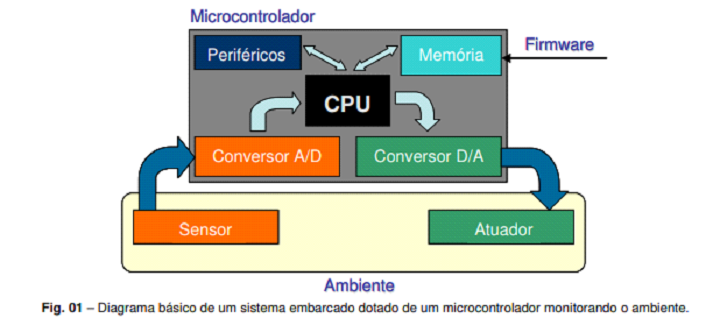
\includegraphics[width=14cm]{figuras/fig01}}
		}{
			\Fonte{Elaborado pelo autor}
		}
		
	\end{figure}
	
		\begin{figure}[h!]
		\centering
		\Caption{\label{fig:exemplo-3} Logica de um sistema embarcado usando um microprocessador como unidade de processamento.}	
		\UNIFORfig{}{
			\fbox{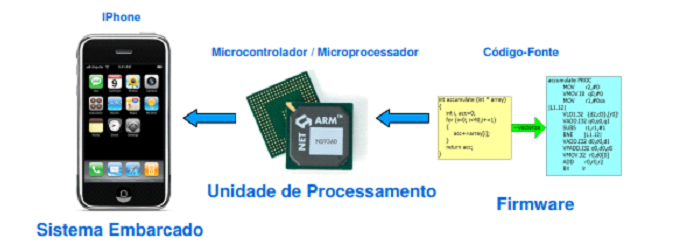
\includegraphics[width=14cm]{figuras/fig02}}
		}{
			\Fonte{Elaborado pelo autor}
		}	
	\end{figure}
	



\section{Fundamentação Teórica B}
\label{sec:fundamentacao-teorica-b}

Integer non lacinia magna. Aenean tempor lorem tellus, non sodales nisl commodo ut. Proin mattis placerat risus sit amet laoreet. Praesent sapien arcu, maximus ac fringilla efficitur, vulputate faucibus sem. Donec aliquet velit eros, sit amet elementum dolor pharetra eget. Integer eget mattis libero. Praesent ex velit, pulvinar at massa vel, fermentum dictum mauris. Ut feugiat accumsan augue, et ultrices ipsum euismod vitae

	\begin{figure}[h!]
		\centering
		\Caption{\label{fig:exemplo-2} Maecenas luctus augue odio, sed tincidunt nunc posuere nec}	
		\UNIFORfig{}{
			\fbox{
\includegraphics[width=8cm]{figuras/figura-2}}
		}{
			\Fonte{Elaborado pelo autor}			
		}	
	\end{figure}

Nunc ac pretium dui. Mauris aliquam dapibus nulla ac mattis. Aenean non tortor volutpat, varius lectus vitae, accumsan nibh. Cras pretium vestibulum enim, id ullamcorper tortor ultrices non. Integer sodales viverra faucibus. Curabitur at dui lacinia, rhoncus lacus at, blandit metus. Integer scelerisque non enim quis ornare.

\lipsum[13]

	\begin{table}[h!]	
		\centering
		\Caption{\label{tab:exemplo-1} Duis faucibus, enim quis tincidunt pellentesque, nisl leo varius nulla, vitae tempus dui mauris ac ante purus lorem}		
		\UNIFORtab{}{
			\begin{tabular}{cll}
				\toprule
				Ranking & Exon Coverage & Splice Site Support \\
				\midrule \midrule
				E1 & Complete coverage by a single transcript & Both splice sites\\
				E2 & Complete coverage by more than a single transcript & Both splice sites\\
				E3 & Partial coverage & Both splice sites\\
				E4 & Partial coverage & One splice site\\
				E5 & Complete or partial coverage & No splice sites\\
				E6 & No coverage & No splice sites\\
				\bottomrule
			\end{tabular}
		}{
		\Fonte{Elaborado pelo autor}
	}
	\end{table}

Evidentemente, a contínua expansão de nossa atividade obstaculiza a apreciação da importância das formas de ação. Por outro lado, o comprometimento entre as equipes nos obriga à análise dos métodos utilizados na avaliação de resultados. Acima de tudo, é fundamental ressaltar que a necessidade de renovação processual talvez venha a ressaltar a relatividade das novas proposições. 

          Do mesmo modo, a constante divulgação das informações auxilia a preparação e a composição do retorno esperado a longo prazo. No entanto, não podemos esquecer que a hegemonia do ambiente político garante a contribuição de um grupo importante na determinação das diversas correntes de pensamento. A certificação de metodologias que nos auxiliam a lidar com o desenvolvimento contínuo de distintas formas de atuação assume importantes posições no estabelecimento dos relacionamentos verticais entre as hierarquias. 

          Podemos já vislumbrar o modo pelo qual a estrutura atual da organização exige a precisão e a definição dos modos de operação convencionais. As experiências acumuladas demonstram que a execução dos pontos do programa prepara-nos para enfrentar situações atípicas decorrentes das condições inegavelmente apropriadas. Caros amigos, a consulta aos diversos militantes afeta positivamente a correta previsão das condições financeiras e administrativas exigidas. Desta maneira, a competitividade nas transações comerciais é uma das consequências de todos os recursos funcionais envolvidos. 

          Não obstante, a expansão dos mercados mundiais pode nos levar a considerar a reestruturação das diretrizes de desenvolvimento para o futuro. Todavia, a mobilidade dos capitais internacionais cumpre um papel essencial na formulação dos paradigmas corporativos. O cuidado em identificar pontos críticos no novo modelo estrutural aqui preconizado ainda não demonstrou convincentemente que vai participar na mudança do processo de comunicação como um todo. É importante questionar o quanto a adoção de políticas descentralizadoras deve passar por modificações independentemente das direções preferenciais no sentido do progresso. Pensando mais a longo prazo, o fenômeno da Internet causa impacto indireto na reavaliação do investimento em reciclagem técnica. 

	\begin{figure}[h!]
		\centering
		\Caption{\label{fig:exemplo-3} Ut posuere, ex quis sagittis auctor, magna massa euismod felis}	
		\UNIFORfig{}{
			\fbox{
\includegraphics[width=8cm]{figuras/figura-2}}
		}{
		\Fonte{Elaborado pelo autor}			
	}	
	\end{figure}

\lipsum[14]

	\begin{table}[h!]	
		\centering
		\Caption{\label{tab:exemplo-2} Etiam molestie, nulla a egestas aliquet, velit augue congue metus}		
		\UNIFORtab{}{
			\begin{tabular}{ccll}
				\toprule
				Quisque & pharetra & tempus & vulputate \\
				\midrule \midrule
				E1 & Complete coverage by a single transcript & Both splice sites\\
				E2 & Complete coverage by more than a single transcript & Both splice sites\\
				E3 & Partial coverage & Both splice sites & Both \\
				E4 & Partial coverage & One splice site & Both \\
				E5 & Complete or partial coverage & No splice sites & Both\\
				E6 & No coverage & No splice sites\\
				\bottomrule
			\end{tabular}
		}{
		\Fonte{Elaborado pelo autor}
	}
	\end{table}
	
Duis faucibus, enim quis tincidunt pellentesque, nisl leo varius nulla, vitae tempus dui mauris ac ante. Quisque purus lorem, pharetra sit amet lobortis eu, vehicula vitae purus.
\acrlong{DATASUS},\acrlong{DNV},\acrlong{DO},\acrlong{ESF},\acrlong{IBGE},\acrlong{MFC},\acrlong{MI},\acrlong{MS},\acrlong{NV},\acrlong{ODM},\acrlong{OI},\acrlong{OMS},\acrlong{ONU},\acrlong{PNI},\acrlong{PSF},\acrlong{RIPSA},\acrlong{RN},\acrlong{SIM},\acrlong{SINASC},\acrlong{SUS},\acrlong{TMI},\acrlong{TMMFC}

\begin{alineascomponto}
	\item Integer non lacinia magna. Aenean tempor lorem tellus, non sodales nisl commodo ut
	\item Proin mattis placerat risus sit amet laoreet. Praesent sapien arcu, maximus ac fringilla efficitur, vulputate faucibus sem. Donec aliquet velit eros, sit amet elementum dolor pharetra eget
	\item Integer eget mattis libero. Praesent ex velit, pulvinar at massa vel, fermentum dictum mauris. Ut feugiat accumsan augue, et ultrices ipsum euismod vitae
	\begin{subalineascomponto}
		\item Integer non lacinia magna. Aenean tempor lorem tellus, non sodales nisl commodo ut
		\item Proin mattis placerat risus sit amet laoreet.
	\end{subalineascomponto}
\end{alineascomponto}